%%
%% This is file `sample-sigconf.tex',
%% generated with the docstrip utility.
%%
%% The original source files were:
%%
%% samples.dtx  (with options: `sigconf')
%% 
%% IMPORTANT NOTICE:
%% 
%% For the copyright see the source file.
%% 
%% Any modified versions of this file must be renamed
%% with new filenames distinct from sample-sigconf.tex.
%% 
%% For distribution of the original source see the terms
%% for copying and modification in the file samples.dtx.
%% 
%% This generated file may be distributed as long as the
%% original source files, as listed above, are part of the
%% same distribution. (The sources need not necessarily be
%% in the same archive or directory.)
%%
%% The first command in your LaTeX source must be the \documentclass command.
\documentclass[sigconf]{acmart}
\usepackage{graphicx}
\usepackage{enumitem} 
\usepackage{float}
\usepackage{mathtools}
\usepackage{booktabs} % For prettier tables
\usepackage{tabularx}
\usepackage{multicol}
\usepackage{unicode-math}
\usepackage{caption}
\usepackage[demo]{graphicx}
%
\makeatletter
\setlength{\@fptop}{0pt}
\makeatother
%
\captionsetup[figure]{labelfont={bf},labelformat={default},labelsep=period,name={Fig.}}
% \usepackage[]{algorithm2e}
% \usepackage[linesnumbered,ruled,vlined]{algorithm2e}
\usepackage[ruled,vlined,linesnumbered]{algorithm2e}    
\newcommand\mycommfont[1]{\footnotesize\ttfamily\textcolor{purple}{#1}}
\SetCommentSty{mycommfont}
\SetKwInput{KwInput}{Input}                % Set the Input
\SetKwInput{KwOutput}{Output}              % set the Output
\settopmatter{printacmref=false}
\setcopyright{none}
\renewcommand\footnotetextcopyrightpermission[1]{}
\pagestyle{plain}
%%
%% \BibTeX command to typeset BibTeX logo in the docs
\AtBeginDocument{%
  \providecommand\BibTeX{{%
    \normalfont B\kern-0.5em{\scshape i\kern-0.25em b}\kern-0.8em\TeX}}}

%% Rights management information.  This information is sent to you
%% when you complete the rights form.  These commands have SAMPLE
%% values in them; it is your responsibility as an author to replace
%% the commands and values with those provided to you when you
%% complete the rights form.
% \setcopyright{acmcopyright}
% \copyrightyear{2018}
% \acmYear{2018}
% \acmDOI{10.1145/1122445.1122456}

%% These commands are for a PROCEEDINGS abstract or paper.
% \acmConference[Woodstock '18]{Woodstock '18: ACM Symposium on Neural
%   Gaze Detection}{June 03--05, 2018}{Woodstock, NY}
% \acmBooktitle{Woodstock '18: ACM Symposium on Neural Gaze Detection,
%   June 03--05, 2018, Woodstock, NY}
% \acmPrice{15.00}
% % \acmISBN{978-1-4503-XXXX-X/18/06}



% Submission ID.
%% Use this when submitting an article to a sponsored event. You'll
%% receive a unique submission ID from the organizers
%% of the event, and this ID should be used as the parameter to this command.
%%\acmSubmissionID{123-A56-BU3}

%%
%% The majority of ACM publications use numbered citations and
%% references.  The command \citestyle{authoryear} switches to the
%% "author year" style.
%%
%% If you are preparing content for an event
%% sponsored by ACM SIGGRAPH, you must use the "author year" style of
%% citations and references.
%% Uncommenting
%% the next command will enable that style.
%%\citestyle{acmauthoryear}

%%
%% end of the preamble, start of the body of the document source.
\begin{document}
\fancyhead{}  % Part of Camera-ready style; Copied from http://www.scomminc.com/pp/acmsig/ccs3.htm#L

%%
%% The "title" command has an optional parameter,
%% allowing the author to define a "short title" to be used in page headers.
\title{Trace Oddity: Methodologies for Data-Driven Traffic Analysis on Tor}

%%
%% The "author" command and its associated commands are used to define
%% the authors and their affiliations.
%% Of note is the shared affiliation of the first two authors, and the
%% "authornote" and "authornotemark" commands
%% used to denote shared contribution to the research.
\author{Somaye Hoseinpur}
 \affiliation{%
   \institution{Brandenburg University of Technology}
}
\email{somaye.hoseinpur@b-tu.de}
%%
%% By default, the full list of authors will be used in the page
%% headers. Often, this list is too long, and will overlap
%% other information printed in the page headers. This command allows
%% the author to define a more concise list
%% of authors' names for this purpose.
% \renewcommand{\shortauthors}{Trovato and Tobin, et al.}

%%
%% The abstract is a short summary of the work to be presented in the
%% article.




\begin{abstract}
One of the main goals of the Tor network is to protect the privacy of internet users by hiding their IP address by encrypting the traffic in multiple layers and transmitting it through a chain of nodes. Although Tor provides user anonymization, traffic analysis can be conducted on the Tor network. Therefore traffic analysis attacks still remain an area of interest for researchers who study traffic and analyze it. The reason for this is that Tor does not introduce delay and dummy traffic. By collecting the traffic from both ends of the communication, client to entry node and exit node to the destination server, an attacker can run the deanonymization process of Tor users by comparing two ends of the communication, this method is known as flow correlation. Like many domains, deep learning techniques are also used in current research on Tor and have improved the performance rates of traffic analysis attacks on this advanced network. In this paper, a state-of-the-art end-to-end (E2E) traffic correlation attack on Tor in a real-world setting has been studied by a novel experimental setup. Contrary to prior works, where a single proxy for collecting network traffic was utilized, the new approach provided by this paper uses several proxies placed at different geographical regions for collecting exit traffic, resulting in more realistic E2E round-trip times and significant degradation of traffic correlation attack performance on realistic timings. To ensure reliable and informative evaluations, a general scientific methodology is developed for the replication and comparison of machine and deep-learning attacks on Tor. The evaluation highlights the importance of the multi-proxy data collection setup and the novel dataset.
\end{abstract}


%%
%% The code below is generated by the tool at http://dl.acm.org/ccs.cfm.
%% Please copy and paste the code instead of the example below.
%%
\begin{CCSXML}
<ccs2012>
 <concept>
  <concept_id>10010520.10010553.10010562</concept_id>
  <concept_desc>Computer systems organization~Embedded systems</concept_desc>
  <concept_significance>500</concept_significance>
 </concept>
 <concept>
  <concept_id>10010520.10010575.10010755</concept_id>
  <concept_desc>Computer systems organization~Redundancy</concept_desc>
  <concept_significance>300</concept_significance>
 </concept>
 <concept>
  <concept_id>10010520.10010553.10010554</concept_id>
  <concept_desc>Computer systems organization~Robotics</concept_desc>
  <concept_significance>100</concept_significance>
 </concept>
 <concept>
  <concept_id>10003033.10003083.10003095</concept_id>
  <concept_desc>Networks~Network reliability</concept_desc>
  <concept_significance>100</concept_significance>
 </concept>
</ccs2012>
\end{CCSXML}

% \ccsdesc[500]{Computer systems organization~Embedded systems}
% \ccsdesc[300]{Computer systems organization~Redundancy}
% \ccsdesc{Computer systems organization~Robotics}
% \ccsdesc[100]{Networks~Network reliability}

%%
%% Keywords. The author(s) should pick words that accurately describe
%% the work being presented. Separate the keywords with commas.
\keywords{end-to-end traffic correlation, traffic analysis, data collection, anonymity, deep learning}

\settopmatter{printfolios=true}

%% This command processes the author and affiliation and title
%% information and builds the first part of the formatted document.
\maketitle


\section{Introduction} \label{1}


Tor \cite{TheOnionRouter} is the most popular anonymization network that hides users’ IP addresses during web browsing by passing the web traffic through a chain of nodes and encrypting the data in multiple layers. There are three types of nodes for each connection: entry node, middle node, and exit node (see Figure~\ref{fig:1}). Each time a user tries to connect to Tor, the user chooses the entry node first and then chooses two more nodes as the middle node and exit node for user. The combination of these three nodes forms a circuit in the Tor network. The data originating from the user is transmitted through this circuit until reaching the web server \cite{privacyguides}. The only point on the path between the user and its final destination that is not encrypted by the Tor algorithm is the connection between the exit node and the server. An adversary can analyze the traffic in this specific connection and get the content. This is only feasible if the user only uses \texttt{HTTP}, in the case of \texttt{HTTPS} the connection between the exit node and the server will be encrypted \cite{Torprojecthttps}.

One of the known attacks that can expose Tor users' identity via traffic analysis is E2E traffic correlation/confirmation. By eavesdropping on the traffic on both ends of a communication, an attacker can use statistical methods of correlation to compare the two sets of information, one from the client to the entry node and another from the exit node to the web server. This attack can be successful if similarities are found between observed traffics, in this case, it can be concluded that both data flows are correlated. For this purpose, an adversary can use different types of metadata captured from the traffic, such as the size and timing of packets \cite{JanThesis}. This is described in detail in Section \ref{2.2}.

E2E traffic correlation based on deep learning is studied in this paper. To run this attack on Tor, the traffic information needs to be captured on both ends of the communication, between the Tor client and entry node and between the exit node and the destination server. These two streams of data are used to deanonymize the users by correlating the data. To this end, an experimental setup is used to run the attack and collect the datasets needed to analyze the attack. However, the main challenge in this setup is capturing the traffic between the exit node and the destination. Due to privacy concerns and the risk of exposing real Tor users' data, the traffic between the exit node and the destination servers should be collected carefully. A common solution to this problem is using a proxy between the exit node and the server as done in prior work \cite{nasr2018deepcorr}. This proxy acts as an intermediary that not only reroutes the traffic that has been generated in this setup but also captures the data. As a result, the need to have direct access to the exit node and the destination server can be eliminated. 

\begin{figure}[h]
  \centering
  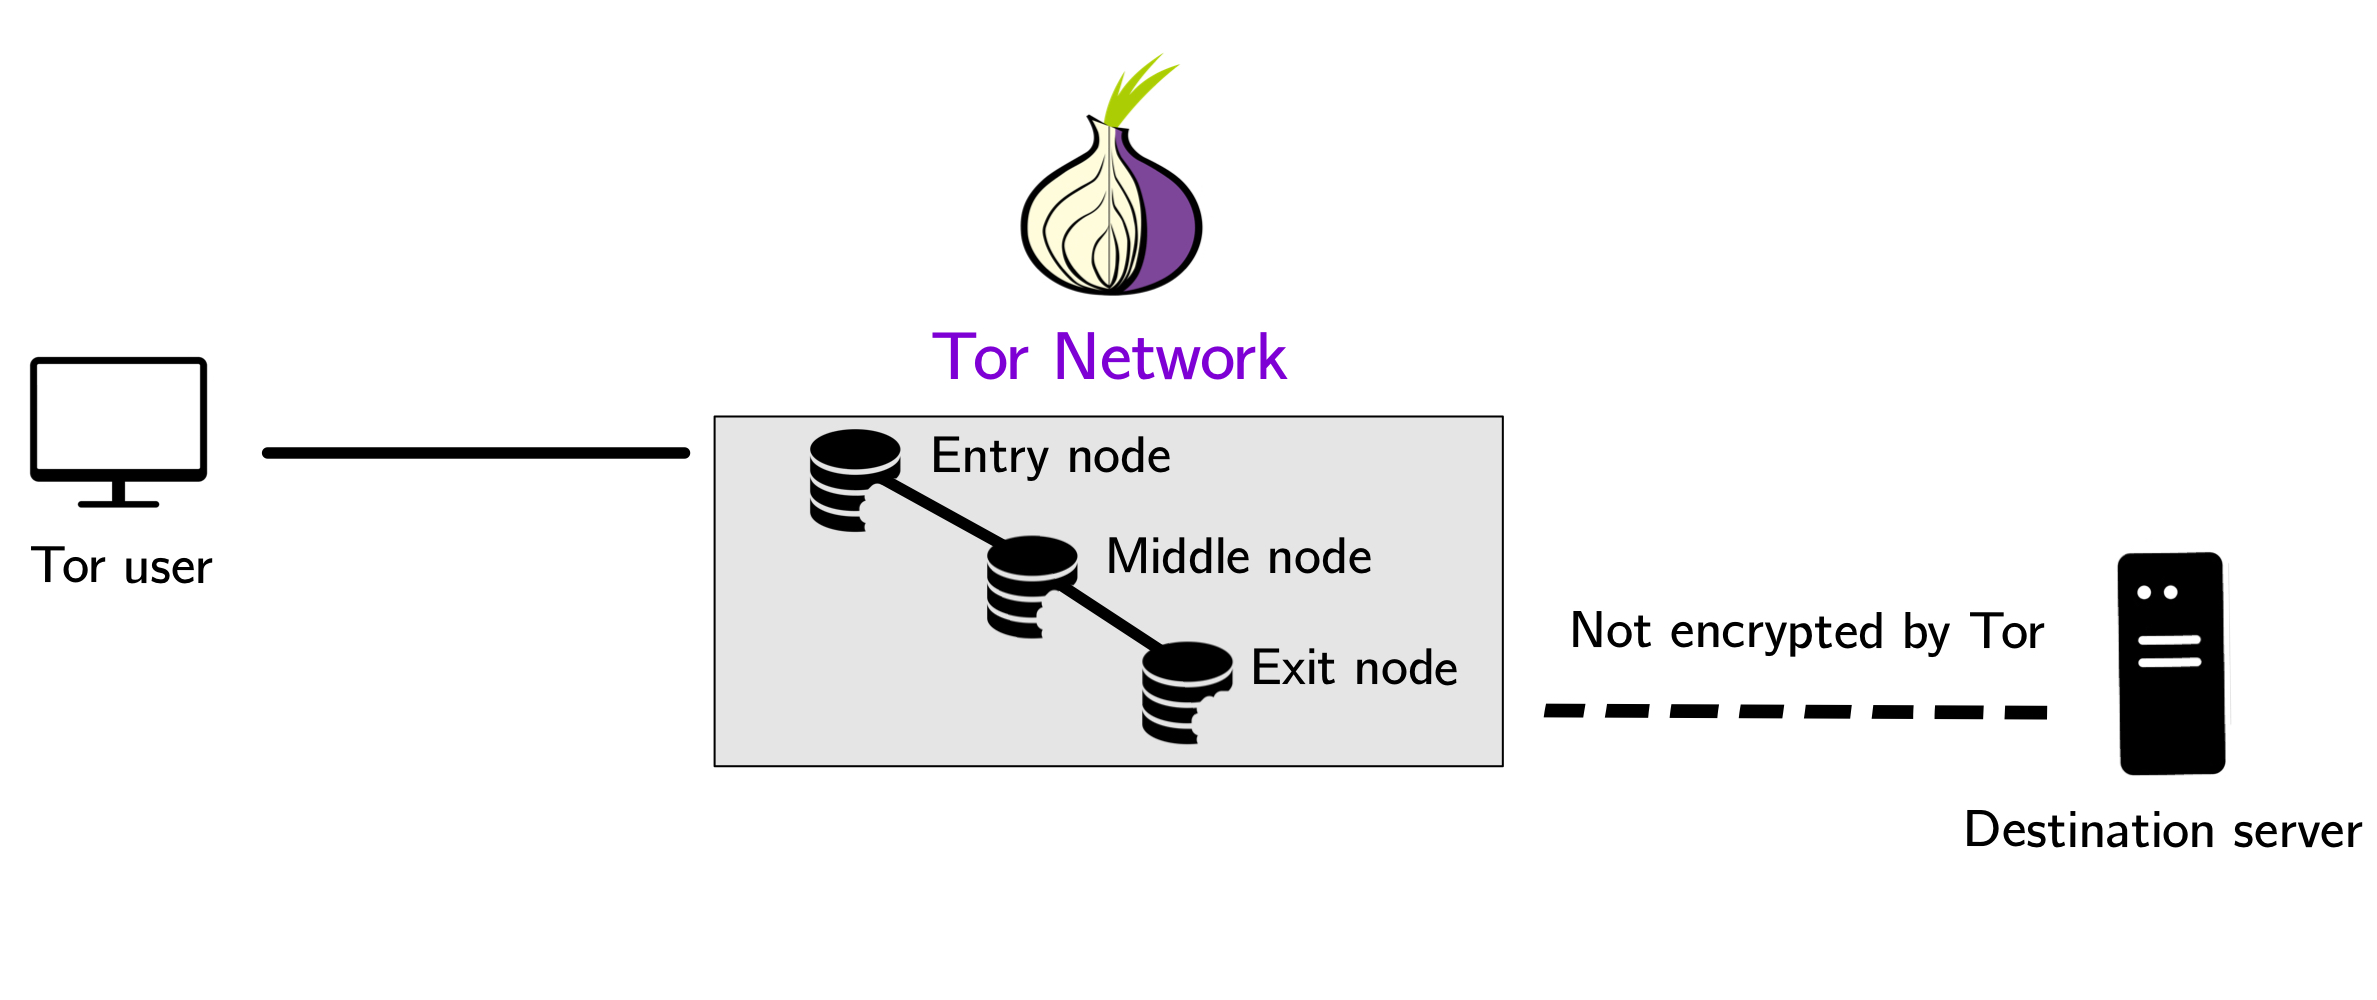
\includegraphics[width=9cm]{Figure_1.jpeg}
 \caption{\textmd{An overview of the Tor network}}
 \label{fig:1}
\end{figure}


The usage of this proxy in attack simulation and its implications are studied in this paper. However, there are issues when using a single proxy at a fixed location. For instance, for the large set of connections in the Tor network, this proxy would be an extra intercontinental hop depending on where it is located geographically in the world. This will eventually cause timing overhead. The timing along with the packet sizes are the main traffic characteristics that an adversary uses to conduct E2E traffic correlation. Another challenge with experimenting with the attack in this setup is the nature of deep learning algorithms. While deep learning performs greater work in E2E traffic analysis attacks on Tor, it comes with the demand for more computational power and, thus, high costs to be able to produce a result with higher success rates. 


In the method proposed in this paper, the impact of the quality of the collected research dataset on E2E traffic correlation attacks has been analyzed. First, in contrast to prior works, the new data collection setup proposed in this paper makes use of a multi-proxy technique to reduce the timing overhead. These multiple proxies are distributed worldwide near the Tor exit nodes. Additionally, a state-of-the-art attack, DeepCorr \cite{nasr2018deepcorr}, that can correlate Tor connections is being evaluated on the new dataset which is introduced in this paper. DeepCorr relies on an advanced deep-learning technique to correlate two sets of traffic flows. Basically, this technique tries to find similarities between two traffic flows to eventually find out a specific user connection. This can be done by pairing the characteristics of packets such as timing and the size of the packets in both traffic flows.

The new experimental setup proposed in this paper is capable of reducing timing bias which was the main drawback of experimental setups applied in prior work \cite{nasr2018deepcorr}. In a summary, this paper provides three  main contributions: 


\begin{enumerate}[label=(\roman*)]

\item \textbf{Novel Multi-Proxy Setup:} This paper proposes a new experimental setup relying on multiple proxies instead of a single proxy. In particular, 14 different proxies have been set up in different locations around the world to gather the traffic after the exit node. This approach reduces the timing overhead of prior work \cite{nasr2018deepcorr} and introduces a more realistic timing measurement.

\item \textbf{Attack Replication Methodology:} The E2E traffic correlation attack, DeepCorr, is used for the purpose of valid comparison between two datasets, one dataset is gathered from using only a single proxy and another is collected by using multiple proxies. The reason for this is to understand whether this setup has any impact on the feasibility of traffic correlation attacks in the real world. The goal of the proposed algorithm in this paper is to reduce the evaluation bias.

\item \textbf{Evaluation Results:} The revisited evaluation of DeepCorr provided in this paper shows the decreased performance of the multi-proxy setup. Considering the difference in average precision results of both datasets which are 7.95\%. This means that an E2E correlation attack using a multi-proxy setup is more difficult which is similar to the real-world situation where an attacker would have a challenging time running the attack. 

\end{enumerate}

\vspace{2mm}

The rest of the paper is organized as follows: \textit{Section \ref{2}} provides an overview of background information regarding the Tor network and its operation and also the motivation for this paper. In \textit{Section \ref{3}}, related work is presented. \textit{Section \ref{4}} discusses the challenges of collecting data. In \textit{Section \ref{5}}, the new data collection setup is explained. In \textit{Section \ref{6}}, the evaluation methodology of the new approach is presented. \textit{Section \ref{7}} presents the evaluation results. \textit{Section \ref{8}} discusses the limitations of the current work and the paper is concluded in \textit{Section \ref{9}}.
\\~\\

\begin{figure*}[h!]
  \centering
  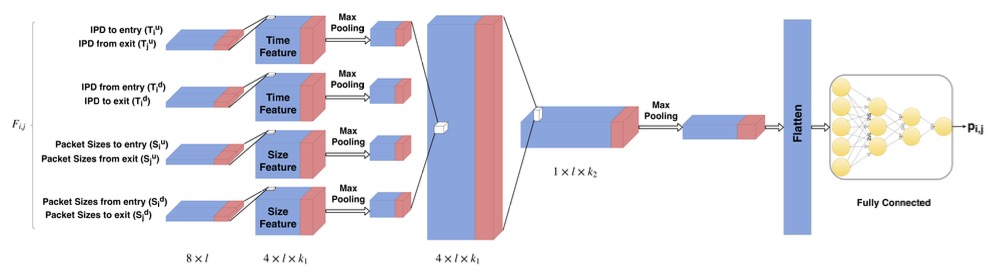
\includegraphics[width=15cm]{Figure_2.jpeg}
  \caption{\textmd{An overview of DeepCorr's convolutional neural network (taken from \cite{nasr2018deepcorr}).}}
  \label{fig:2} 
\end{figure*}

\vspace{-6mm}

\section{Background} \label{2}

Here, the technical information about the operation of Tor and the main types of traffic analysis attacks against Tor, specifically E2E traffic correlation which this paper focuses on, are provided. 


\subsection{Circuits and Connections} \label{2.1}

In Tor, the user does not directly connect to the destination website/server. Instead, the connection goes through a path, called a circuit. The circuit, which is built by the user, consists of three nodes, known as entry, middle, and exit. Before building the circuit, the Tor user connects to one of the directory authorities which are redundant and trusted servers set up by the Tor Project, to get the list of available nodes in the network. Then, the Tor user chooses an entry node and extends the path further to the middle and exit nodes. The user requests are then three times encrypted using three different session keys and are sent over the three nodes. Using Diffie-Hellmann Key Exchange protocol, a Tor user and nodes can generate a shared secret key that is used for encryption and decryption of the traffic data. Each of the nodes can decrypt only one layer of encryption. With the decryption of the last layer by the exit node, the data/request will be sent to the destination server/website \cite{Torprojectoverview}. If the website the user is visiting supports encryption of web traffic, the data passing from the exit node to the server is also encrypted. Otherwise, an adversary can access sensitive information or try to deanonymize the user. 

Although the selection of nodes is random, there are requirements for choosing them. Only the nodes that are stable and fast can be chosen as the first node. Each node can have a different kind of responsibility at the same time and serve multiple clients simultaneously. For example, a node can be an entry node for a client and an exit node for another client. Since Tor provides the IP addresses of nodes publicly available, governments can block these IP addresses to prevent users from connecting to the Tor network and thus have anonymity. To overcome this problem, Tor provides the possibility to connect to a specific type of nodes called bridges. The information about bridges is not available publicly, so they cannot be easily blocked \cite{Torprojectrelays}. 


\subsection{Traffic Analysis Attacks on Tor} \label{2.2}

Traffic analysis attacks against Tor are possible due to Tor's network design and traffic patterns that it generates. Thus, an adversary can analyze the traffic passing through the network and extract the sensitive information. E2E traffic correlation is a type of attack against Tor in which the attacker observes both ends of Tor connection to identify the similarities in the traffic and, thus, correlates a Tor user and its destination. This is done by gathering traffic from the exit node to the server, (this is usually meta-data which consists of timing and packet size characteristics), and from the client to its entry node \cite{defendingtorcorrelation}.

Another kind of attack against the Tor network is website fingerprinting. In this attack, the adversary monitors the traffic entering and leaving the exit node and identifies the patterns in the traffic that can be associated with specific websites. The attacker creates a dataset by crawling websites in the Tor network prior to the attack and then feeds this dataset to machine learning for comparing this data to the information he gathered from monitoring the connection between the client and the entry point to predict the website that user wants to visit \cite{277132}.

In this paper, a new dataset consisting of network traffic collected using multiple proxies has been introduced. This dataset is used to evaluate the feasibility of E2E traffic analysis attack based on a deep learning technique.

\vspace{3mm}

\section{Related work} \label{3}

The research in this paper is mainly based on DeepCorr \cite{nasr2018deepcorr}, which is the first traffic correlation attack that utilizes deep learning. Deep learning is a technique that is long-established for its performance and has been used in many research areas such as protocol detection \cite{oh2017p,rimmer2017automated}, encrypted video stream analysis \cite{schuster2017beauty}, and deducing different encrypted traffic \cite{aceto2018mobile}. Also, the challenges of this technique have been investigated by Arp et al. \cite{arp2022and}.


DeepCorr uses an advanced deep learning architecture that learns flow correlation function which can be conducted on Tor traffic. Using the convolutional neural networks (CNNs) \cite{ConvolutionalNetworks}, the flow correlation system of DeepCorr takes traffic flow data such as packet size, direction, and timing as the input and uses them to derive features. Each traffic flow F is represented as \emph{F= [$T^{u}$,$T^{d}$,$S^{u}$,$S^{d}$]} where $T$ is inter-packet delays, $S$ is packet sizes, $u$ is uplink (client to server), and $d$ is downlink directions (server to client) of traffic flow. The deep learning attack correlates a pair of traffic segments $F_{i}$ ($i$ is intercepted by a Tor entry guard) and $F_{j}$ ($j$ is intercepted by a controlled exit node). This pair of traffic flows can be represented as follow: 
\begin{equation*}
\emph{$F_{i,j}$= [$T_{i}^u$,$T_{j}^u$,$T_{i}^d$,$T_{j}^d$,$S_{i}^u$,$S_{j}^u$,$S_{i}^d$,$S_{j}^d$]} 
\end{equation*}


As shown in Figure~\ref{fig:2}, DeepCorr's architecture uses a fully connected neural network with three layers and two convolution layers. The rationale behind using the first convolution layer is to identify the association between adjacent rows in the input matrix $F_{i,j}$, which should be associated with correlated Tor flows, such as between $T_{i}^u$ and $T_{j}^u$. The second convolution layer in DeepCorr is responsible to identify traffic features by combining timing and size features. After the second convolution layer, the resulting output is flattened and passed through a fully connected network that has three layers. In order to maintain permutation invariance and prevent overfitting \cite{Overfitting}, DeepCorr applies max pooling after each convolutional layer. The final outcome of the network is:
\begin{equation*}
\emph{$\rho_{i,j}$= \Psi($F_{i,j}$)} 
\end{equation*}


This output is utilized to determine the correlation between the two input flows in $F_{i,j}$. In order to normalize the network output, a sigmoid function is applied that rescales the output values between zero and one. This means that \emph{$\rho_{i,j}$} provides the probability of correlation between flows $i$ and $j$, for example, if they are the start and end of the same Tor connection.

The authors of DeepCorr assessed the effectiveness of flow correlation using true positive rate (TPR) and false positive rate (FPR). True positive rate refers to the proportion of associated flow pairs that DeepCorr correctly identifies as correlated, where $i$ and $j$ represent segments of the same Tor connection. The false positive rate measures the fraction of non-associated flow pairs that DeepCorr mistakenly identifies as correlated, such as when $i$ and $j$ represent segments of different Tor connections. To evaluate FPR, DeepCorr matches every collected entry flow to every collected exit flow, resulting in $\emph{N × (N - 1)}$ false correlations for each experiment, where $N$ is the number of test flow pairs in the experiment.



Although DeepCorr is more effective than previous methods of flow correlation, the authors of this paper performed a critical evaluation of its performance using a more realistic research setup. They modified the DeepCorr's implementation\footnote{https://github.com/woodywff/deepcorr} to be used in this experiment to provide new insights on evaluating, tuning, scaling, and explaining the deep learning-based attack. Another research group, Oh et al. \cite{oh2022deepcoffea}, recently proposed a different type of correlation attack called DeepCoFFEA that uses metric learning techniques. DeepCoFFEA employs the triplet network architecture as a feature extractor and splits flows into windows, and extracts features for each window, enabling multiple semi-independent correlation tests that can be combined to increase the differences between matched and unmatched pairs of flows and reduce false positives. Since the authors of this work used different learning approaches, future work can be evaluating the performance of their attack based on the datasets that the current paper has provided. 

\vspace{3mm}

\section{Challenges of Data Collection} \label{4}

In reality, one can sniff the Tor exit traffic with the aim of traffic analysis by using a proxy between the exit node and the web server. However, if proxies are used, an additional hop is added to the connection that might impact the timing characteristics of the captured traffic. By analyzing a state-of-the-art E2E attack \cite{nasr2018deepcorr}, it can be argued that using a single proxy causes timing overhead. As a result, these timing alterations impact the traffic traces captured from different circuits. It is worth stating that, usually an attacker would not use any proxy to gather traffic. Instead, they will  directly collect the traffic traces from the exit node in the circuit.

\subsection{Measurement Setup and Overview} \label{4.1}

In order to test the timing characteristic of traffic collected from the proxy, a client has been configured to initiate a Tor connection with the aim of gathering round-trip times (RTTs). This is done by visiting the top 100 websites of the Tranco list \cite{pochat2018tranco} \footnote{https://tranco-list.eu/list/4L8X} through 15,935 Tor circuits consisting of three nodes. At last, the RTTs from these web servers to the websites are gathered by sending an HTTP HEAD request and recording how long it takes till the user gets the response. In the following, the result of timing measurements in the setup is discussed. 

\subsection{Analysis of RTT Measurements} \label{4.2}

In order to analyze the impact of using single and multiple proxies on the timing properties of the collected Tor traffic, the following steps have been done. First, the differences in timing from the client to the single proxy located in the U.S. among the group of proxies are examined. Then the timings that are obtained from two different proxy configurations are compared, namely a single proxy in the U.S. and one proxy among the 14 different proxies in the data centers. Finally, the extra time that is introduced in the timing based on the number of proxies within the set of 14 proxies is measured. 

\vspace{3mm}

\subsubsection{Inter-continental Connections}

The authors of this paper argue that evaluating the attack using only one proxy to relay the traffic data between the exit node and server has a great impact on the RTT of the captured traffic. This can cause some problems in the process of performing the attack using deep learning. In the prior work of Nasr et al \cite{nasr2018deepcorr}, they used only one proxy in the U.S. and the exit nodes were mostly located in Europe. However, this causes timing overhead from an extra hop at the end of the connection. This problem can be seen after gathering and comparing the collected timings at both endpoints between the client and the website. For this analysis, only the circuits whose nodes are located in Europe or North America are considered. These circuits represent about 96\% of all collected circuits (15,935). Since the clients are located in Europe, their connection to the proxies in the U.S. includes one or many inter-continental hops, as shown in Table~\ref{tab:table1}. As a result, the single-proxy setup introduces an extra hop of transmission between Europe and North America. This can cause problems for the feasibility of the traffic analysis due to the fact that it affects the RTT between the client and proxy.

\vspace{3mm}

\subsubsection{Single Proxy vs. Multiple proxies vs. No Proxy}
Here, the evaluation of the RTTs for all websites in the dataset using all Tor circuits is provided. For this purpose, three different proxy configurations have been used: (i) a single proxy that is located in the eastern U.S. which was also used in the prior work by Nasr et al \cite{nasr2018deepcorr}; (ii) 14 proxies from which the proxy that is near to the exit relay in a Tor circuit is always chosen, (iii) and no proxy, where the measured RTT is the exact measurement that an attacker would obtain in the real-world attack scenario. In each setting, the authors collect: (i) timing characteristics from each Tor circuit to each proxy (ii) timing in the connection of each Tor circuit to each website without using a proxy, and (iii) the timings from each proxy to each website. Finally, the impact of different proxy setups is analyzed.
In Figure~\ref{fig:3}, the distribution of end-to-end RTTs in the three different setups is shown. The timings in multi-proxy setup and no-proxy setup are very similar.


\begin{table}[H]
  \begin{center}
    \begin{tabular}{S|S|S}
      \toprule % <-- Toprule here
      \textbf{Hops} & \textbf{Single Proxy} & \textbf{Multi-Proxy} \\
      % $\alpha$ & $\beta$ & $\gamma$ \\
      \midrule % <-- Midrule here
      0 & - & 8,653 (54.3\%)\\
      1 & 10,811 (67.8 \%) & 2,158 (13.5 \%)\\
      2 & - & 4,131 (25.9\%)\\
      3 & 4,468 (28.0 \%) & 337 (2.1 \%)\\
      \bottomrule % <-- Bottomrule here
    \end{tabular}
    \caption{\textmd{The single (U.S.) proxy setup introduces an extra inter-continental connection (based on \cite{RimmerV}).}}
    \label{tab:table1}
  \end{center}
\end{table}


\begin{figure}[h]
  \centering
  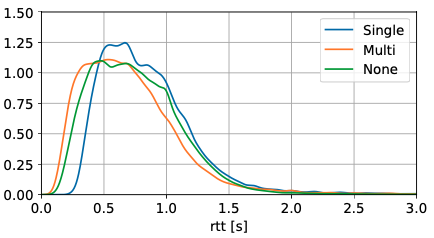
\includegraphics[width=8cm]{Figure_3.png}
 \caption{\textmd{RTTs measured between clients and websites for three different proxy setups (taken from \cite{RimmerV}).}}
 \label{fig:3}
\end{figure}


\subsubsection{Number of Proxies}
For the purpose of reducing timing overhead, the number of proxies needed to be used should be considered. Choosing a proxy near to the web server impacts in favor of decreasing the timing overhead. Here, the impact of using multiple proxies on the transmission overhead is discussed. In this setup, random proxies from 14 available proxies have been selected and then the distance between the exit node and the nearest proxy to it is measured. If only one proxy in a circuit is used, the average minimum distance is 5,700km. If 5 proxies are used, the distance reduces to 1,000km, and in a case where all 14 proxies are used, the distance reduces to 500 km. This result is shown in Figure~\ref{fig:4} with the blue line. 

\begin{figure}[h]
  \centering
  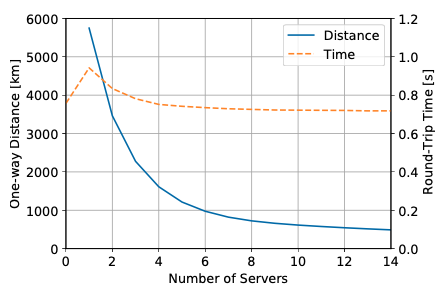
\includegraphics[width=8cm]{Figure_4.png}
 \caption{\textmd{Differences in distance and RTTs when using a different number of available proxies for choosing one for each circuit (taken from \cite{RimmerV}).}}
 \label{fig:4}
\end{figure}

In addition to the distance, the timing overhead is also measured. According to the results shown in Figure \ref{fig:4}, in the setup with no proxy the average RTT is 0.75 seconds. While the average RTT in the single-proxy setup is 0.94 seconds, which means 190ms timing overhead. As the number of proxies increased up to 14, the RTT value is similar to the RTT value of the no-proxy setup. In conclusion, using only one proxy to capture traffic from an exit node to a web server causes timing overhead. The timing characteristic of Tor traffic is one of the main features that is used in E2E traffic correlation and, thus, it should be reduced, which can be done by using multiple proxies in the experimental setup.

\vspace{3mm}


\section{Experimental Setup for Data Collection} \label{5}

In this section, the configuration and the structure of the new experimental setup for performing E2E traffic analysis attacks are provided.

\subsection{Requirements} \label{5.1}

Since the prior E2E traffic analysis attack is based on deep learning techniques \cite{nasr2018deepcorr}, in this work it is also required to feed the algorithm with a dataset to train and the deep-learning algorithm. Thus, a dataset has to be prepared consisting of traffic information from the client to the entry node and also from the exit node to the web server.

 However, recording this information would expose real Tor users. To avoid this, proxies are used at the exit node. The proxy acts as a tunnel to forward the information from the exit relay to the web server. Instead of using a single proxy as done in prior work \cite{nasr2018deepcorr}, several proxy servers are used. To this end, there are several requirements to consider while choosing the proxies.

\vspace{3mm}

\textbf{Circuit diversity:} It is possible that in one browsing session, Tor changes the circuit and creates a new one. In most cases, the entry node in different circuits remains the same, but the middle and exit node is switched. Circuit characteristics such as the length and bandwidth differ for each circuit. Due to the fact that Tor nodes are distributed across the world, each circuit connection has its own special performance, including the length of the connection and the amount of bandwidth. By using a proxy, it is possible to keep the original circuit connection. 

\vspace{3mm}

\textbf{Server locations:} Tor users can visit various websites whose web servers are distributed at different locations across the world. As a result, the distance between the exit node and the web server may vary. In the new experimental setup, several proxies at different locations are distributed and, thus, the chance of being near either an exit node or a web server is increased. The goal is to avoid additional hop during the E2E correlation attack.  

\vspace{3mm}

\textbf{Onion server traffic:} In a normal situation in the Tor network when the request is being transmitted from the client to the server, the server can identify that this request comes from the Tor network. Hence, it may redirect the user to the corresponding .onion address. Then, the client will initiate the connection to the relevant onion service. In a situation, where a proxy is the last node that transmits the information to the web server, the client does not establish a connection to any onion service. 

\subsection{Setup Overview} \label{5.2}

The experimental setup implemented in \cite{RimmerV} consists of three main sections: clients which are configured to run on a virtual machine, a central management entity that manages the website crawling to collect data and orchestrates \texttt{tcpdump}, and an extra proxy between exit nodes and web servers to capture the network traffic on the other side of Tor connections, as shown in Figure~\ref{fig:5}.

\begin{figure}[h]
  \centering
  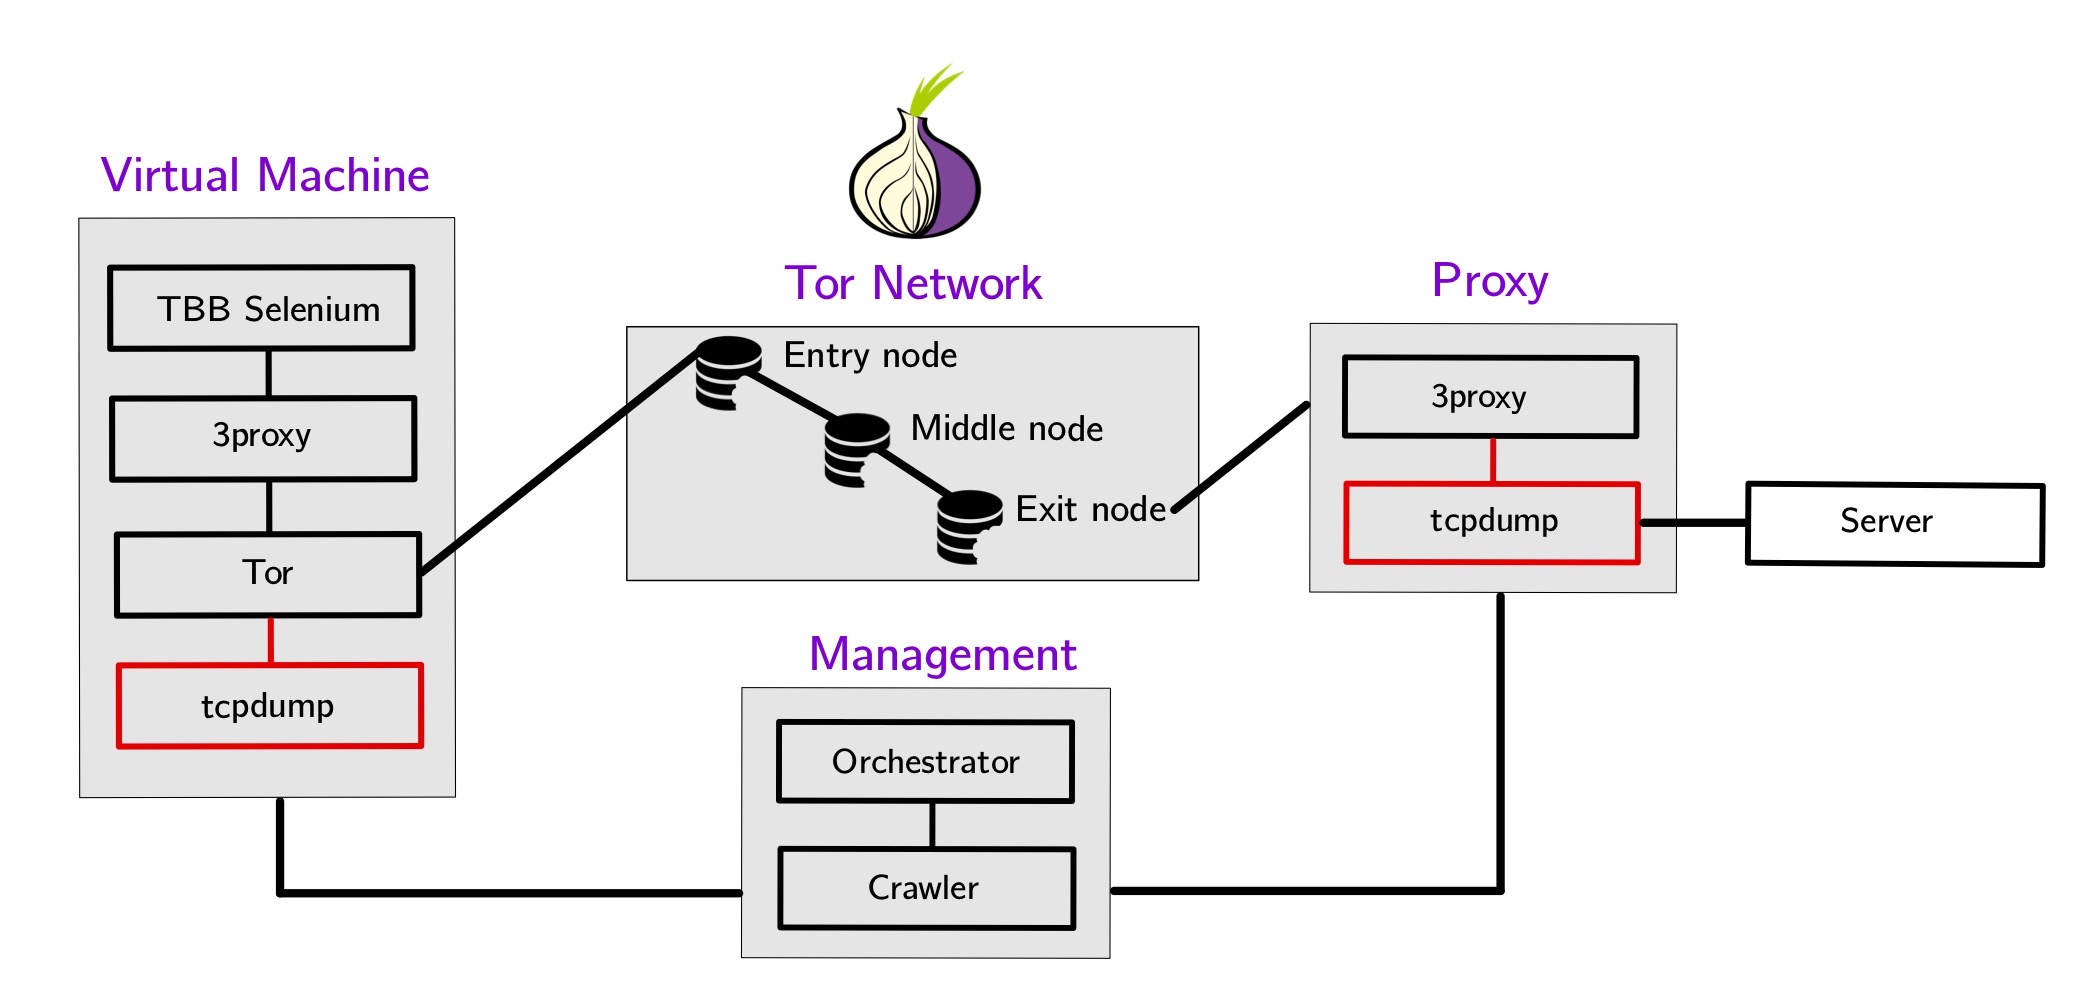
\includegraphics[width=8.5cm]{Figure_5.jpg}
 \caption{\textmd{Experimental setup (based on \cite{RimmerV}).}}
 \label{fig:5}
\end{figure}

Each client in this setup consists of Tor Browser Bundle (TBB), \texttt{3proxy}, and the core Tor implementation that creates a circuit, and \texttt{tcpdump} which is being used to capture the traffic between the client and entry node. The central management system is responsible for arranging the website crawling and coordinates the \texttt{tcpdump} on both traffic monitoring points. The \texttt{3proxy}\footnote{https://3proxy.ru} which is a simple and efficient software tool that functions as both a proxy client and server is also configured in this setup. Using \texttt{3proxy}, it is possible to forward traffic to the additional proxy that is put between the exit node and the web server. To overcome the problem of the additional hop, 18 proxies are set up in 6 different locations (London, San Francisco, New York, Amsterdam, Singapore, and Frankfurt). The authors chose different geographical locations for the proxies with the hope that some of them can be near any exit node or web server. 

By placing an additional proxy between the exit node and the web server, it is not possible to record the traffic since the circuit has been built in advance and the data coming from the client will be redirected to the web server without tunneling through the additional proxy. To this end, the authors must place their own \texttt{SOCKS5} node after the initial proxy, which establishes the connection between the Tor client and the entry node. Additionally, they are required to create a chain of proxies on a particular port, which Tor will later utilize for establishing the connection. By doing so, the authors can control the circuit creation such that they would be able to choose the correct node candidates from the set of available nodes for the user. Eventually, they can determine the closest optimal proxy to the exit node of the circuit, create the proxy chain on the port designated for use by Tor, and wait for the connection to be established.

From a technical point of view, the authors have to modify the Tor client to be able to identify the appropriate circuit connection. This alternation is the replication of the original Tor's circuit selection process that controls port implementation by scanning all current circuits and choosing three nodes that are most probable to be selected for the next connection. This process helps the authors to employ the IP address of the exit node to enable access to the proxy for incoming connections. An extra advantage of this configuration is that any other connection to the proxy is eliminated, only the controlled circuit and connection are connected. A drawback for this configuration would be if an incorrect circuit is predicted on the client side, an incorrect proxy is chosen for this circuit (and therefore a false proxy location), then the incoming connection to the proxy uses a different IP address and, thus, is blocked at the proxy.

\subsection{Data Collection Details} \label{5.3}

Three different datasets have been gathered by using the experimental setup described above. For the collection of the first two datasets, the 15,000 most popular websites from the Tranco Top 1 million sites \cite{pochat2018tranco}\footnote{https://tranco-list.eu/list/KW8W} were used. The information utilized for these two datasets was gathered in 23 days. Only one proxy was used for the $SD$ dataset in one Amazon data center and for the $MD$ dataset, several proxies in six Amazon data centers have been used. The data for the ${MD}$$_{1mln}$ dataset, which is the largest and final dataset, is collected in 8 days using visiting the same websites in the Tranco list. 


\section{Evaluation Methodology} \label{6}

The goal of configuring this novel data collection setup is to know whether it affects the feasibility of traffic correlation attacks. In this setup, DeepCorr \cite{nasr2018deepcorr} - a state-of-the-art E2E traffic correlation attack - is evaluated with the collected datasets. Since the $SD$ dataset has been collected by only one proxy and the $MD$ dataset by multiple proxies, the performance of DeepCorr in different settings can be analyzed.

Moreover, in order to have a valid comparison between two datasets, there are several factors that should be considered when evaluating data-driven attacks, such as selecting appropriate performance metrics, implementing a proper attack replication algorithm to evaluate deep learning models on new data, and conducting an explainability analysis. If these factors are incorporated, then it can be guaranteed that any differences in attack performance come from semantic differences in the data not from interpretation or chance. This is very crucial, especially for attacks that are dependent on deep neural networks that rely heavily on randomness. Further details on each of these factors of the evaluation methodology are explained in the following section.


\subsection{Performance Metrics} \label{6.1}

The goal of the scientific empirical evaluations of traffic analysis attacks against Tor is to approximate the extent to which Tor users' privacy is at risk. However, such attacks are simulated in lab conditions under a set of simplified assumptions, which brings technically feasible performance estimation but limits the realism of the attacks. The performance evaluation of the E2E traffic correlation that can happen in the real world is very difficult to perform in lab conditions. Previous studies have focused on the estimation of the performance of website fingerprinting attacks in relation to real-world challenges \cite{juarez2014critical,wang2020high}. In this paper, the main focus is to have a realistic measurement for the E2E correlation attack by using the new data collection setup. In a simplified research setting, the exact choice of metrics and the correct interpretation of results are important. This paper examines the metrics used by the state-of-the-art and suggests improvements.

In the previous study, the authors used the False Positive Rate (\textit{FPR}) and True Positive Rate (\textit{TPR}), also known as Recall, to estimate the E2E correlation performance. (\textit{FPR}) represents the rate of non-associated pairs that were incorrectly predicted as correlated, while (\textit{TPR}) represents the rate of truly associated pairs that were correctly predicted as correlated. Nevertheless, these metrics do not reflect the full capability of the attacker in real-world scenarios and could be misleading. The reason for this is the base rate fallacy specific to E2E attacks. This problem comes from the inherent imbalance of positive and negative pairs in the test set. The attacker must correlate all combinations of traces (N × N), while only 1 out of N intercepted connections is truly associated. Therefore, even a high (\textit{TPR}) and a low (\textit{FPR}) do not necessarily make the attack reliable. This indicates that using (\textit{FPR}) and (\textit{TPR}) to estimate performance in E2E attacks is insufficient.

It is important to report all relevant metrics to provide transparent and informative estimations. Therefore, depending on the attacker's goals and the costs of false positives and false negatives, one may choose to optimize the precision-recall trade-off to obtain a more trustworthy detector. Previous work optimized the attack based on loss, but for DeepCorr, there is no theoretical guarantee that the optimal loss corresponds to the optimal precision-recall trade-off. Therefore, an adversary may also evaluate a domain-specific metric on every training epoch in addition to the standard loss. In this paper, the authors addressed this disconnect by optimizing for Average Precision (AP), which summarizes the area under the PR-curve.



\subsection{Attack Replication} \label{6.2}

The performance of the E2E correlation attack is analyzed twice, each time with one of the datasets, the one collected from using a single proxy and the other dataset collected from using multiple proxies. Suppose a higher performance of the E2E correlation attack is obtained using the dataset that belongs to a single proxy. In that case, it means that the timing characteristics of the attack have a positive impact on attack simulation. Also if a lower attack performance is obtained by using the dataset that belongs to multiple proxies, then it means that traffic correlation using multiple proxies is much more challenging. Through experimental analysis, the authors get the performance of the attack, which will indicate the quality of the datasets. To properly evaluate the E2E correlation attack on the new datasets, the authors of this paper developed an attack replication algorithm. Further details on the important steps of the Algorithm \ref{alg:replication} are discussed in the following section.

\vspace{4mm}

\begin{algorithm}
\caption{Replication of DeepCorr on two datasets. AP is the target metric and \textit{t}-test is used for statistical significance (taken from \cite{RimmerV}).}
\label{alg:replication}
\SetKwInOut{Input}{input}\SetKwInOut{Output}{output}
\Input{Datasets $D_{1}$ and $D_{2}$, ML/DL attack \emph{A}, hyperparameter search space \emph{S.} }
\Output{Dataset with highest mean attack performance, the difference between means; statistical significance}
Set number of cross-validation folds \emph{K}

Set maximum number of attack configurations \emph{C}

Set number of randomized training runs \emph{n}

$AP_{D_1}$ \gets \{\} ,  \State $AP_{D_2}$ \gets \{\}
\DontPrintSemicolon
\SetKwFunction{FLoop}{Loop}
\SetKwProg{Fn}{for}{}{}
\BlankLine

\SetKwFor{RepTimes}{repeat}{times}{end}
    
\For{dataset $d \in \{\ $D_{1}$ , $D_{2}$ $ \}\ } {

    Split \emph{d} into \emph{K} equal folds $d_{1,...,K}$
    
    \For{ $k \in \{\ 1,...,K \}\ $ } {
        Put aside fold $d_{k}$ as $test_{k}$

        Assign the remaining folds to $train_{K}$

        Sample $tune_{K}$  \subseteq  $train_{K}$

        \State $AP_{best}$  \gets 0
    
        \For{ $i \in \{\ 1,...,C \}\ $ } {
            Sample config $c_{i}$ from \emph{S} using the chosen optimization strategy

            Split $tune_{k}$ into $tune_{train} , tune_{val}$ 

            Train \emph{A} with config $c_{i}$ on $tune_{train}$

            Compute \emph{AP} on $tune_{val}$

            \If {$AP > AP_{best}$} {
                $c_{k} = c_{i} , AP_{best} = AP $
            }
        }
        \RepTimes{n} {
        
            Change random seed
            
            Train \emph{A} with config $c_{k}$ on $train_{k}$
            
            Compute \emph{AP} on $test_{k}$
            
            \State $AP_{d}$ \gets $AP_{d}$ \cup \emph{AP} 
        }
        
    }
}

Compute \emph{t-test} and \emph{p-value} on ($AP_{D_1}$ , $AP_{D_2}$)

\KwRet {$argmax (\overline{\rm AP}_{D_1} , \overline{\rm AP}_{D_1}) ; |  \overline{\rm AP}_{D_1} - \overline{\rm AP}_{D_2}| ; \emph{p-value.}$ }
\end{algorithm}

\vspace{4mm}




\textbf{Hyperparameter Tuning:} This process is very important and has to be done separately for each dataset. This ensures that each dataset is evaluated using the best model configuration and hyperparameters and, thus, provides a fair comparison. This is necessary for two reasons, firstly, because it reflects the procedure used by real-world attackers, and secondly, because the best configuration allows for a more accurate assessment of the dataset's ability to capture the relevant characteristics.

Additionally, the limitation of resources as the algorithm entails numerous complex iterations through the datasets has to be considered. There should be a balance between having a comprehensive evaluation and ensuring a reasonable computation time. In terms of tuning in the algorithm, the necessary resources primarily depend on the size of the search space (S), the maximum number of evaluated attack configurations (C), and the size of a subset of training data selected for tuning (step 10), which could be a fraction or the entire set. It is worth stating that employing a uniform optimization approach is very important for the algorithm since it decides the hyperparameter configuration to be assessed at each iteration which is shown in step 13 of the algorithm \ref{alg:replication}. The most popular optimization strategies are Grid search (comprehensive search), Random search, and Bayesian optimization (probabilistic search). The authors in this paper utilized Bayesian optimization and opted to start with a basic model and progressively augment its complexity. 

\vspace{3mm}

\textbf{Cross-Validation:} In order to prevent selection bias, which could occur from testing on only one set of data, the algorithm employs a technique similar to k-fold cross-validation. This process includes using several subsets of the dataset for training, validating, and testing the model on multiple iterations \cite{GeneralizationError}. This technique can assure that the results are consistent and generalize well across the different subsets. On the other hand, if the outcome is not consistent across the different subsets, it may indicate an inconclusive result.

\vspace{3mm}

\textbf{Randomization:} This should also take into consideration that deep neural networks are not completely deterministic. This means that they can produce different results for the same input, even though everything else is constant. Non-determinism may happen due to random weights and biases in the neural network, or randomly selecting the data while training \cite{Randomness}. The authors address this issue by performing multiple runs for cross-validation fold with different random seeds. By doing so, they can get a better estimate of the model's performance and its consistency across different data and weight initialization, thus, evaluating the stability of the attack. 

\vspace{3mm}

\textbf{Statistical Significance:} The algorithm eventually gives the dataset that produced a higher-ranked result of attack performance. However, in order to indicate the reliability of the results, the statistical significance has to be evaluated. This is very important since relying only on reporting the best runs without considering statistical significance could be random. The authors address this by performing a two-sample t-test to compare the performance of data-driven models with equal variances \cite{StatisticalSignificance}.



\subsection{Explainability Analysis} \label{6.3}

The replicated algorithm is designed in a way that ensures the accuracy of comparison between using a single-proxy dataset versus multiple-proxy dataset. The goal is to indicate which one of these datasets is more difficult to attack, which as a result would determine whether one of the datasets is better than the other. Nevertheless, since deep neural networks are complex and very hard to understand, it is challenging to make definite decisions based only on numerical performance metrics. Therefore, an extra explainability analysis is performed by the authors to explain the result of the two attack models and, thus, strengthen the output of the evaluation. To perform the explainability analysis, the authors used a technique called visualization of the activation maps, which is a technique that is typically used for image classification in Convolutional Neural Networks (CNNs) \cite{ConvolutionalNetworks}. Using this method, the authors can understand which part of the traffic best fits the correlation attack, since it is applied on the first layer of the neural network, where the input is still understandable.

The authors focus more on the output of the first convolutional layer that produces a set of 2D activation maps by taking the inner product of a chunk of the input trace and kernel. To identify the important areas in the original input, the highest activation values are used due to the fact that the size of each activation map is proportional to the size of the input trace. More precisely, in order to determine which areas in the traffic data are more important to the model for correlation, this process has to be repeated across all activation maps in the first layer and also average the result across multiple input traces. Finally, the authors report the findings by performing this analysis individually for associated and non-associated pairs in each dataset. 


\section{Evaluation Results} \label{7}

The proposed methodology by the authors of this paper is used in this section to compare the performance of the state-of-the-art E2E correlation attack on the collected datasets. This includes hyperparameter tuning and cross-validation with training and testing. The input format is the same as the one used in prior work that evaluated the attack which is discussed in (related work). Finally, the report of the main performance results, scalability results on the larger dataset, and explainability analysis achieved through visualization of activation maps are provided in the following sections.



\subsection{Attack Replication { }---{ } Tuning} \label{7.1}


This section of the evaluation focuses on the hyperparameter tuning part of the Algorithm \ref{alg:replication} (steps 10-18). These parameters determine the performance of the machine learning model and a correct combination of hyperparameters can increase the detection rate of the algorithm \cite{weerts2020importance}. Hyperparameter tuning is applied for each of datasets $SD$ and $MD$ and two different search spaces are conducted, the one proposed in prior work, \( \mathcal{DC} \) (DeepCorr) \cite{nasr2018deepcorr}, and the one which has been modified for use in this paper \( \mathcal{TDC} \) (Tiny DeepCorr). The difference between \( \mathcal{TDC} \) and \( \mathcal{DC} \) is the number of kernels in each convolutional layer. As it is shown in Table ~\ref{tab:table3}, in \( \mathcal{TDC} \) the number of kernels in the first convolutional layer is reduced from 2000 to 64 or 128, and the second layer from 800 to 128 kernels. This approach resulted in increasing the training speed from 9 hours of training time to 20 minutes and 13 hours of testing time to 40 minutes.
In order to analyze the timing and size features individually, the original kernel size (2,30),(4,10), and strides (2,1)(4,1) of the \( \mathcal{DC} \) model have been kept the same. Typically, kernel size is a matrix of numbers that are multiplied with the input image with the aim of producing a feature map. Its size refers to the dimensions of the window used for the convolutional process. Strides indicate the step size for the sliding window used while performing convolution. Both hyperparameters control the feature extraction and spatial resolution of a convolutional neural network \cite{Convolution_Arithmetic}.



The next step is to modify the $N_{neg}$ parameter, which sets the number of non-associated pairs used as negative examples during network training for each truly associated pair. In general, there are two sets of pairs in this paper: a set of associated flow pairs or ($F_{i}, F_{j}$) which consist of two segments of the same Tor connection. The other set of flow pairs is non-associated flow pairs (or negative samples) that consist of two Tor flows that each belong to a different Tor connection \cite{nasr2018deepcorr}. If $N_{neg}$ is smaller, it decreases the available training data, and larger $N_{neg}$ negatively impacts learning by causing an imbalance between positive and negative samples. The authors address this issue by using a $weighted$ loss function that adjusts the learning process by adding a class weight value to the loss function to reduce errors in the truly-associated pairs. To compensate for the data imbalance during training, the authors adjust the $w_{p}$ parameter, which is the weight of the positive class, within the range of 1 (standard non-weighted loss) to $N_{neg}$ (a fully balanced loss). $lr$ ow learning rate is also defined by the authors which indicate the rate at which the optimization algorithm updates the weights of the neural network during training to achieve better performance and fast convergence. Table~\ref{tab:table2} shows all the resulting search space for \( \mathcal{TDC} \) model. Columns 3 and 4 of this table show the final optimal configurations that are chosen for both datasets based on the highest results from AP.


According to Figure~\ref{fig:7}, it can be observed that the evaluation of \(\mathcal{TDC} \) model on $SD$ dataset has higher performance compared to $MD$. The authors denote that $MD$ required more kernels in the first convolutional layer, thus, higher learning capacity is needed. Moreover, they indicate that according to the Hyperparameter tuning experiment, the task of learning becomes more challenging when working with the $MD$ dataset.


\subsection{Attack Replication { }---{ } Training and Test} \label{7.2}


The authors apply 5-fold cross-validations such that for each fold, 80\% of correlated flow pairs with $N_{neg}=49$ negative samples and 20\% of flow pairs that belong to positive samples, are trained and validated. Overall, the number of truly associated flow pairs is $N = 7,948$ for both $SD$ and $MD$ datasets. Also, for each fold, the evaluation is repeated three times ($n=3$) with random initialization. So the final number of runs for both $SD$ and $MD$ datasets is $k\times\ n=15$. The average precision is used for early stopping which is a method to avoid overfitting by stopping the training process at points that the learning degraded. For this purpose, the weights that resulted in higher AP are obtained. 



The final performance metrics are shown in Table~\ref{tab:table4}. Based on the AP results, the E2E attack correlation on $SD$ is more successful. To balance the model's performance in identifying both positive and negative pairs, the authors optimized $Pr$ (precision) metric individually for a low False Positive Rate (FPR) of 0.001 to minimize the rate of false positives and a high True Positive Rate (TPR) of 80\% to maximize the rate of true positives. TPR of \(\mathcal{TDC}\)$_{SD}$ is 47.76\% and TPR of \(\mathcal{TDC}\)$_{MD}$ is 32.43\%. The difference between these rates is 15.33\% which shows the TPR rate decrease for $MD$ dataset. On the other hand, FPR rate for \(\mathcal{TDC}\)$_{MD}$ increases which indicates higher false positives for this dataset. 





\begin{table}[h]
  \begin{center}
    \begin{tabular}{l|l|l|l}
      \toprule % <-- Toprule here
      \textbf{Hyperp.} & \textbf{Search space} & \( \mathcal{TDC} \)$_{SD}$ & \( \mathcal{TDC} \)$_{MD}$ \\
      % $\alpha$ & $\beta$ & $\gamma$ \\
      \midrule % <-- Midrule here
      kernels & [[64],[128], & [64,128] & [64,128]\\
              & [64,64],[128,128]] &  &  \\
      pool size & \{3,5\} & 5 & 5\\
      dense layers & [[1000],[500,100],  & [500,100] & [500,100]\\
                   &  [1000,100]] &   &  \\
      optimizer & { }---{ } & Adam & Adam\\
      lr & \{0.001,0.0001\} & 0.0001 & 0.0001\\
      batch size & [32,64,128] & 32 & 64\\
      dropout & [0.0,0.4,0.6] & 0.6 & 0.6\\
      $w_{p}$ & [1,2,5,25] & 5 & 5\\
      $N_{neg}$  & [9,49,199] & 49 & 49\\
      \bottomrule % <-- Bottomrule here
    \end{tabular}
    \caption{\textmd{Optimal hyperparameters for the \( \mathcal{TDC} \) models on single- and multi-proxy datasets (taken from \cite{RimmerV}).}}
    \label{tab:table2}
  \end{center}
\end{table}

\vspace{-6mm}

\begin{table}[h]
  \begin{center}
    \begin{tabular}{l|l|l|l}
      \toprule % <-- Toprule here
      \textbf{Hyperparam} & \textbf{Search space} & \( \mathcal{TDC} \)$_{SD}$ & \( \mathcal{TDC} \)$_{MD}$ \\
      % $\alpha$ & $\beta$ & $\gamma$ \\
      \midrule % <-- Midrule here
      kernels & [2000,800] & [64,128] & [64,128]\\
      pool size & \{3,5\} & 5 & 5\\
      dense layers & [[2000],[2000,500]] & [500,100] & [500,100]\\
      optimizer & { }---{ } & Adam & Adam\\
      lr & \{0.001,0.0001\} & 0.0001 & 0.0001\\
      batch size & [32,64,128] & 32 & 64\\
      dropout & [0.0,0.4,0.6] & 0.6 & 0.6\\
      $w_{p}$ & [1,2,5,25] & 5 & 5\\
      $N_{neg}$  & [9,49,199] & 49 & 49\\
      \bottomrule % <-- Bottomrule here
    \end{tabular}
    \caption{\textmd{Hyperparameters of the \( \mathcal{DC} \) model on multi-proxy dataset and the optimal hyperparameters for \( \mathcal{TDC} \) on both datasets (taken from \cite{RimmerV}).}}
    \label{tab:table3}
  \end{center}
\end{table}



% \\~\\

\begin{table*}[ht]
  \centering
  \begin{tabular}{lcccccc}
  \toprule[1.5pt]
  \head{\textbf{Model}} & \head{$AP_{val}$ (\%)} & \head{$AP_{test}$ (\%)} & \head{$TPR_{FPR=0.001}$ (\%)} & \head{$Pr_{FPR=0.001}$ (\%)} & \head{$FPR_{TPR=80\%}$} & \head{$Pr_{TPR=80\%}$}\\
  \midrule
  $\(\mathcal{TDC}\)$$_{SD}$ & 79.22 \pm 6.80 & 24.55 \pm 6.98 & 47.76 \pm 9.01 & 21.40 \pm 3.27 & 0.0071 \pm 0.003 & 7.68 \pm 2.82 \\
  $\(\mathcal{TDC}\)$$_{MD}$ & 71.27 \pm 9.48 & 13.83 \pm 6.60 & 32.43 \pm 10.59 & 15.02 \pm 5.19 & 0.0154 \pm 0.008 & 4.08 \pm 1.98 \\
  \hline
  $p-value$ & 0.007568 & 0.000028 & { }---{ } & { }---{ } & { }---{ } & { }---{ } \\
  \hline
  $\(\mathcal{TDC}\)$$_{MD-1mln}$ & 95.3 \pm 1.2 & 5.099 \pm 1.22 & 35.93 \pm 2.77 & 39.37 \pm 1.75 & 0.775 \pm 1.12 & 7.09 \pm 2.03 \\
  % \hline
  \bottomrule[1.5pt]
  \end{tabular}
  \caption{\textmd{E2E attack performance of retrained algorithm on both $SD$ and $MD$ datasets (taken from \cite{RimmerV}).}}
  \label{tab:table4}
\end{table*}

\vspace{-1mm}

\textbf{Scalability:} In order to know if the attack would perform well on larger datasets, the authors performed another evaluation of \(\mathcal{TDC}\)$_{MD}$ on 25,000 associated pairs from the $MD$$_{1mln}$ dataset. As stated in Section \ref{5.3}, this is the largest dataset in this paper. The result is shown in Table~\ref{tab:table4}, indicating a decreased performance of the E2E correlation attack. This highlights the fundamental difficulty of E2E correlation attacks where an increase in the amount of intercepted traffic traces leads to a quadratic growth of the test set which leads to overall decreased attack performance.

\vspace{3mm}

\textbf{Results:} In conclusion, based on thorough tuning and evaluation made by the authors, it can be inferred that an E2E correlation attack performs better on $SD$ in comparison to $MD$, which aligns with the author's initial hypothesis. Specifically, the problem with realism in single-proxy data collection setups seems to favorably influence the estimated performance of data-driven E2E attacks. This could be due to the presence of noisy timings in the input, which is examined more with explainability analysis in a further section.


\vspace{4mm}

\textbf{Explainability:} In order to better understand the performance of the attack, the authors compute the mean activations maps of the first convolution layer for both datasets from correlated (positive sample) and non-correlated traffic pairs (negative sample). An example for the differences in the mean activation maps is shown in Figure~\ref{fig:6}. This activation map is created from the first convolutional layer of \(\mathcal{TDC}\) which has a (4,64,271) shape (width, height, and depth) of the filter used to perform the convolution operation.
\vspace{3mm}

\begin{figure}[H]
  \centering
  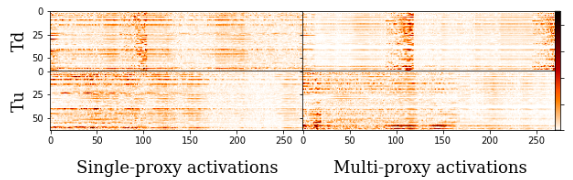
\includegraphics[width=8cm]{Figure_6.png}
 \caption{\textmd{Comparing the computed mean activation maps that are obtained from positive and negative samples of $SD$ and $MD$ datasets (taken from \cite{RimmerV}).}}
 \label{fig:6}
\end{figure}

\vspace{2mm}

The plotted downside of this figure shows the uplink timing ($T^u$) and the upside shows the downlink timing ($T^d$) of the correlated and non-correlated traffic pairs. Darker sides of this map show a higher number of values, which in turn, indicates higher importance. Although the initial assumption was that downlink timing is more important since it includes the server responses, the activation map highlights the uplink timings to be more important. This might be due to the fact that neural networks tend to rely on simpler features, even if more complex predictive patterns are available. To verify this idea, the authors suggest future work based on analyzing and studying the nature and inner parts of deep learning-based E2E correlation attacks, similar to recent studies exploring wireless fingerprinting \cite{DLbasedWF}.


\begin{figure*}[h!]
  \centering
  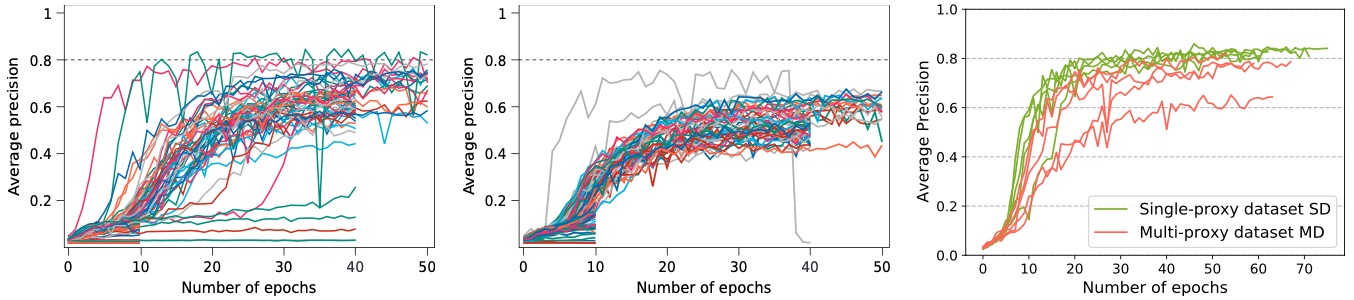
\includegraphics[width=17.5cm]{Figure_7.jpg}
  \caption{\textmd{Hyperparameter tuning of \( \mathcal{TDC} \) separately on both datasets $SD$ (left) and $MD$ (middle) datasets, the left one shows the cross-validation}} (taken from \cite{RimmerV}).
  \label{fig:7} 
\end{figure*}

\vspace{3mm}

\section{Discussion} \label{8}


In this section, the limitation of the current study and future work are discussed. 

\vspace{3mm}

\textbf{Representativeness of Traffic.} In a real-world scenario, users browse not only the homepage but also the other pages of the websites. For the purpose of the experiment in this paper, the datasets that have been collected consist only of the requests for visiting the main homepage of the websites. One reason is comparing these datasets to prior work \cite{nasr2018deepcorr}. Hence, a future work proposed by the authors using a new method to gather a more human-like E2E (and website fingerprinting) dataset and assess the impact of traffic analysis attacks.

\vspace{3mm}

\textbf{Proxy-Related Overhead.} Evaluating the E2E correlation attack with a dataset that has been prepared with a proxy does not endanger the Tor users' privacy. This paper provided a new data collection setup based on a multi-proxy approach that as a result addressed the problem of single-proxy-based data collection. Nevertheless, future work can be analyzing the effect of using proxies on traffic metadata. This analysis would be possible by collecting exit node data of real Tor users. However, reducing privacy concerns of real Tor users can be done by contacting the Tor Research Safety Board\footnote{https://research.torproject.org/safetyboard/}.  

\vspace{3mm}

\textbf{Ethics Considerations.} For realistic analysis of the E2E correlation attack, collecting a dataset that is more similar to Tor's daily transmission traffic data is required. For the purpose of comparison to prior work, a real-world traffic dataset has been collected. However, all of Tor's guidelines for ethical research have been followed thoroughly to not endanger real Tor users' privacy \cite{ethicaltorresearch}.

\vspace{3mm}

\textbf{Defenses Against Traffic Analysis.} The analysis of new data collection in this paper is based on unprotected traffic data. For similar future work, an idea is to evaluate known protection schemes. The authors made the datasets of this work publicly available for this purpose. These datasets are the first that consist of two threat models for both E2E correlation and website fingerprinting attacks that are useful for research on evaluating protection schemes against these attacks.

\vspace{3mm}

\textbf{Onion Services.} Almost any website can be reached through an onion service by using the \texttt{Alt-Svc} response header which is responsible for indicating an alternative service such as onion for future HTTP requests. In this work, the proxies are hosted on a cloud network that provides the connection to the targeted websites. As a result, the websites did not send the Alt-Svc header, and the Tor Browser client did not attempt to access them over the onion service. Additionally, since the Tor Browser utilized a proxy chain, it could not resolve or connect to .onion addresses. This means that the data collection method presented by this paper differs from a real-world scenario where websites would redirect users to an onion service. In a real-world attack, the attacker must consider the differences in requests sent to exit nodes and onion services. The authors conducted preliminary tests and found that onion services are seldom accessed when loading a new website. Nonetheless, investigating the impact of loading resources from onion services on attacks is an important area for future research.

\vspace{-3mm}

\section{Conclusion} \label{9}


In conclusion, this paper presented a new technique for performing data-driven E2E correlation attacks on Tor. The authors introduced a new experimental setup that enables the collection of Tor traffic with more realistic timing characteristics while minimizing additional overhead in proxy-based E2E measurements. Additionally, a replication algorithm with evaluation metrics has been proposed to ensure a fair comparison of data-driven attacks with new datasets. The novel approach of this paper based on the multi-proxy data collection setup provides a more realistic timing characteristic of traffic flow. Although the experiments show that this technique introduces more challenging learning, it is very similar to the real-world scenario of attackers' abilities to perform the attack. Thus, this work can be considered a more realistic E2E correlation attack evaluation. Finally, the research code and the multi-proxy dataset are made available as open source to facilitate further research on traffic correlation and website fingerprinting attacks.



\vspace{5mm}
\\~\\


% \begin{acks}
% To Robert, for the bagels and explaining CMYK and color spaces.
% \end{acks}

%%
%% The next two lines define the bibliography style to be used, and
%% the bibliography file.


\bibliographystyle{ACM-Reference-Format}

\bibliography{literature}


\end{document}
\endinput
%%
%% End of file `sample-sigconf.tex'.
